\documentclass[a4,11pt]{wmecai}
\usepackage{hyperref}
\usepackage[brazil]{babel}
\usepackage[utf8]{inputenc}

%%%%%%%%%%%%%%%%%%%%%%%%%%%%%%%%%%%%%%%%%%%%%%%%%%%%%%%%%%%%%%
%% ARQUIVOS NECESSÁRIOS NO OVERLEAF (além deste .tex):
%%   wmecai.cls    — classe do evento (pasta Template_Artigo)
%%   wmecai.pdf    — logo do evento (pasta Template_Artigo)
%%   cc_by.png     — ícone de licença (pasta Template_Artigo)
%%   fig_pca.png   — graficos/eixo_a/a4_pca.png
%%   fig_b5.png    — graficos/eixo_b/b5_fala_chat.png
%%   fig_c3.png    — graficos/eixo_c/c3_cordas.png
%% Total: 7 arquivos + este .tex
%%%%%%%%%%%%%%%%%%%%%%%%%%%%%%%%%%%%%%%%%%%%%%%%%%%%%%%%%%%%%%

\usepackage{graphicx}
\usepackage[centertags]{amsmath}
\usepackage{indentfirst,amsfonts,amssymb}
\usepackage{booktabs}
\usepackage{cite}
\usepackage{xcolor}   % substitui 'color' — define 'gray' e não conflita com wmecai.cls
\usepackage{url}

\begin{document}

%*************************************************************
\title{Estudo de Audiência Compartilhada no YouTube}

\author{
{\large Janderson Pereira}\thanks{janderson.pereira@usp.br},~
{\large Walter Soares Antonio Junior}\thanks{waltersoares@usp.br},~
{\large Junior Fernandes Marques}\thanks{junior.marques@usp.br},~
{\large Afonso Paiva Neto}\thanks{apneto@usp.br}\\
{\small Universidade de São Paulo (USP) -- Instituto de Ciências Matemáticas e de Computação (ICMC) -- Mestrado Profissional em Matemática, Estatística e Computação Aplicadas à Indústria (MECAI)}\\
}

\criartitulo

%*************************************************************
\section{Introdução}

As mensagens de chat em transmissões ao vivo (\textit{live streams}) no YouTube
expõem a identidade pública do comentarista via \texttt{channel\_id},
permitindo o rastreamento longitudinal de indivíduos entre canais
distintos~\cite{Hamilton2014}. Diferentemente das métricas de consumo
passivo (visualizações, inscritos, \textit{watch time}), esse sinal
constitui evidência de engajamento ativo e rastreável sem coleta de dados
privados.

No jornalismo digital brasileiro, a fragmentação de audiência entre
veículos concorrentes é pouco estudada quantitativamente~\cite{Webster2012}.
Compreender quanto do público é compartilhado tem implicações
para decisões editoriais, planejamento de mídia e inteligência competitiva.

Este trabalho apresenta uma metodologia computacional para medir a
sobreposição de audiência ativa entre 12~canais brasileiros de jornalismo
no YouTube durante 30~dias (20/05/2026 a 20/06/2026), integrando três eixos:
(\textit{i})~dados multivariados por PCA e dendrograma de Ward,
(\textit{ii})~análise textual por TF-IDF, t-SNE e cruzamento fala--chat, e
(\textit{iii})~grafos de similaridade via coeficiente de Jaccard.

Para ter acesso aos códigos, os dados agregados anonimizados e outras visualizações, \href{https://wsoaresjr.github.io/MAI5017-Visualizacao-da-Informacao}{clique aqui para acessar o site} .

%*************************************************************
\section{Metodologia}

\subsection{Coleta e anonimização}

Os dados foram obtidos via YouTube Data API~v3 e \textit{chat replay}
público, cobrindo: metadados de vídeo (título, horário, duração), métricas
de audiência simultânea (CCV), mensagens de chat (texto, \textit{offset},
\textit{super chat}) e transcrições automáticas.
Visando conformidade com a LGPD~\cite{LGPD2018}, nenhum
\texttt{channel\_id} real é persistido: cada identificador é substituído
por SHA-256 com \textit{salt} fixo, preservando a capacidade de unir
registros sem expor dados pessoais.
O recorte final está descrito na Tabela~\ref{tab:dataset}.

\begin{table}[h]
\caption{Estatísticas do conjunto de dados (período 20/05/2026--20/06/2026).}
\centering
\small
\begin{tabular}{lr}
\toprule
\textbf{Grandeza} & \textbf{Valor} \\
\midrule
Canais monitorados        & 12 \\
Transmissões ao vivo      & 2.133 \\
Mensagens de chat         & 1.855.415 \\
Autores únicos            & 98.881 \\
Autores em $\geq$2 canais & 12.374\ \ (12,5\%) \\
\bottomrule
\end{tabular}
\label{tab:dataset}
\end{table}

\subsection{Eixo A — Dados multivariados}

Cada canal é representado por oito métricas padronizadas ($z$-scores):
número de transmissões, total de mensagens, autores únicos, mensagens por
mil visualizações, pico médio de CCV, duração mediana, proporção de
recorrentes e valor total de \textit{super chat}.
A Análise dos Componentes Principais (PCA)~\cite{Wold1987} reduz esse espaço para visualização bidimensional;
o dendrograma hierárquico usa o critério de Ward~\cite{Ward1963}, que
minimiza a variância intra-cluster a cada fusão.
A Figura 1 apresenta a projeção resultante.

\subsection{Eixo B — Documentos e textos}

TF-IDF~\cite{Salton1988} representa as mensagens de chat após remoção de
\textit{stopwords}. A projeção t-SNE~\cite{vanderMaaten2008} posiciona
cada transmissão (25 amostras por canal) de forma que vocabulários
semelhantes apareçam próximos. O cruzamento de frequências entre
transcrições (fala do canal) e chat (Figura 2) quantifica
termos amplificados ou suprimidos pelo público.

\subsection{Eixo C — Grafos de sobreposição}

Seja $A_i$ o conjunto de autores únicos do canal~$i$. O índice de
Jaccard~\cite{Jaccard1912} entre canais $i$ e $j$ é
\begin{equation}
  J(i,j) = \frac{|A_i \cap A_j|}{|A_i \cup A_j|} \in [0,1].
  \label{eq:jaccard}
\end{equation}
A matriz $12\times12$ resultante alimenta um grafo ponderado e o diagrama
de cordas (Figura 3), que evidencia a magnitude e
a distribuição da circulação de público entre canais.

%*************************************************************
\section{Resultados e Discussão}

\begin{figure}
    \centering
    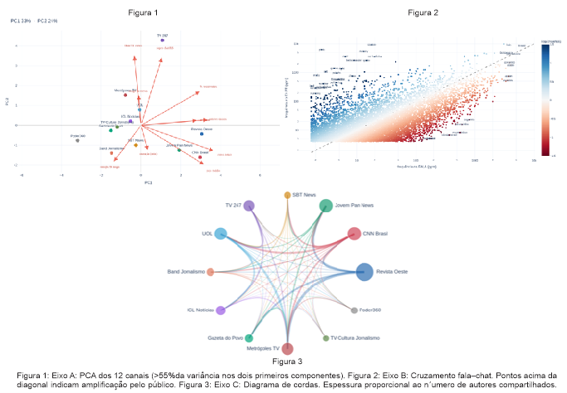
\includegraphics[width=1\linewidth]{Imagem1.png}
    \label{fig:placeholder}
\end{figure}


\textbf{Eixo A.}
O plano PCA (Figura 1) revela três perfis:
(a)~canais de grande alcance e chat intenso
    (CNN~Brasil, Revista~Oeste, Jovem Pan News);
(b)~canais de nicho
    (Poder360, TV~Cultura Jornalismo, Band~Jornalismo); e
(c)~TV~247, isolado pelos altos valores de recorrência de audiência e
\textit{super chat}, padrão reforçado pelo dendrograma de Ward.

\textbf{Eixo B.}
No cruzamento fala--chat (Figura 2), nomes de figuras políticas
(``lula'', ``bolsonaro'', ``moraes'') são, fortemente, amplificados pelo
público em relação à fala dos apresentadores.
Termos de contextualização jornalística (``decreto'', ``processo'')
ficam abaixo da diagonal de equilíbrio --- o chat polariza mais do que
informa, padrão consistente com \textit{live streaming}~\cite{Hamilton2014}.
A projeção t-SNE confirma aglomerados temáticos coerentes com o viés
editorial declarado de cada canal.

\textbf{Eixo C.}
O maior coeficiente de Jaccard foi $J=0{,}0553$ (CNN~Brasil --
Jovem Pan News). Mais de 90\% dos pares apresentou $J<0{,}03$,
indicando públicos predominantemente distintos.
O diagrama de cordas (Figura 3) torna visível que as cordas
mais espessas ligam os três canais de maior alcance, enquanto canais de
nicho (Poder360, TV~Cultura) têm circulação mínima de público.
Ainda assim, 12,5\% dos comentaristas (12.374~indivíduos) circularam
por dois ou mais canais --- fluxo \textit{cross-editorial} estrategicamente
relevante para anunciantes e gestores de programação.

%*************************************************************
\section{Conclusões}

A integração do coeficiente de Jaccard com PCA, dendrograma de Ward,
t-SNE e análise fala--chat permite caracterizar, de forma simultânea e
com baixo custo, sobreposição de público, perfis de engajamento e
proximidade temática entre canais concorrentes. Embora os públicos sejam
majoritariamente segmentados ($J_{\max}=0{,}0553$), a fração de 12,5\%
que circula entre canais é estrategicamente relevante. A metodologia é
replicável para outros nichos e janelas temporais, com alinhamento à
LGPD~\cite{LGPD2018}. Como próximos passos, pretende-se ampliar a janela
temporal, explorar análise de sentimento supervisionada em português e
publicar o \textit{dataset} agregado anonimizado.

Reforçamos a sugestão para que acesse o site para verificar a análise completa, com outras visualizações. \href{https://wsoaresjr.github.io/MAI5017-Visualizacao-da-Informacao}{clique aqui para acessar o site} .

%*************************************************************
\begin{thebibliography}{00}

\bibitem{Hamilton2014}
W.~A. Hamilton, O.~Garretson e A.~Kerne.
Streaming on Twitch: Fostering participatory communities of play
within the live streamed video game ecosystem.
In {\it Proc.\ CHI}, pp.~1315--1324. ACM, 2014.
DOI: 10.1145/2556288.2557048.

\bibitem{Jaccard1912}
P.~Jaccard.
The distribution of the flora in the alpine zone.
{\it New Phytologist}, 11(2):37--50, 1912.
DOI: 10.1111/j.1469-8137.1912.tb05611.x.

\bibitem{LGPD2018}
Brasil.
Lei n.º~13.709, de 14 de agosto de 2018 ---
{\it Lei Geral de Proteção de Dados Pessoais (LGPD)}.
Diário Oficial da União, Brasília, 2018.

\bibitem{Salton1988}
G.~Salton e C.~Buckley.
Term-weighting approaches in automatic text retrieval.
{\it Information Processing \& Management}, 24(5):513--523, 1988.
DOI: 10.1016/0306-4573(88)90021-0.

\bibitem{vanderMaaten2008}
L.~van der Maaten e G.~Hinton.
Visualizing data using t-SNE.
{\it Journal of Machine Learning Research}, 9:2579--2605, 2008.

\bibitem{Ward1963}
J.~H. Ward~Jr.
Hierarchical grouping to optimize an objective function.
{\it Journal of the American Statistical Association},
58(301):236--244, 1963.
DOI: 10.1080/01621459.1963.10500845.

\bibitem{Webster2012}
J.~G. Webster e T.~B. Ksiazek.
The dynamics of audience fragmentation: Public attention in an age
of digital media.
{\it Journal of Communication}, 62(1):39--56, 2012.
DOI: 10.1111/j.1460-2466.2011.01616.x.

\bibitem{Wold1987}
S.~Wold, K.~Esbensen e P.~Geladi.
Principal component analysis.
{\it Chemometrics and Intelligent Laboratory Systems},
2(1--3):37--52, 1987.
DOI: 10.1016/0169-7439(87)80084-9.

\end{thebibliography}

\end{document}
